\documentclass[12pt]{article}

\usepackage[utf8]{inputenc}
\usepackage{latexsym,amsfonts,amssymb,amsthm,amsmath,graphicx,mathtools,subfig,hyperref}
\usepackage[parfill]{parskip}
\usepackage[export]{adjustbox}
\usepackage[justification=centering]{caption}
\usepackage{nameref}

\hypersetup{
    colorlinks=true,
    linkcolor=blue,
    filecolor=magenta,      
    urlcolor=cyan,
}

\DeclareMathAlphabet{\mymathbb}{U}{BOONDOX-ds}{m}{n}

\setlength{\parindent}{0in}
\setlength{\oddsidemargin}{0in}
\setlength{\textwidth}{17cm}
\setlength{\textheight}{22cm}
\setlength{\topmargin}{0cm}
\setlength{\headheight}{0pt}
\setlength{\footskip}{30pt}

\newcommand{\figw}{7cm}
\newcommand{\nnperfw}{7cm}

\title{EE-556 Homework 3}
\author{Edoardo Debenedetti}

\begin{document}

\maketitle

\section{Multiclass classification}

\subsection{Theory}

\subsubsection{Multinomial logistic regression estimator}

\subsubsection{Multinomial logistic regression estimator gradient}

\stepcounter{subsubsection}
\subsubsection{Lipschitz constant}

\subsubsection{\texorpdfstring{$\ell$}{Lg}-1 Proximal operator}

\subsubsection{\texorpdfstring{$\ell$}{Lg}-2 Proximal operator}

\subsection{Handwritten digit classification}

\stepcounter{subsubsection}
\subsubsection{Algorithms implementation and convergence}

\begin{figure}
    \centering
    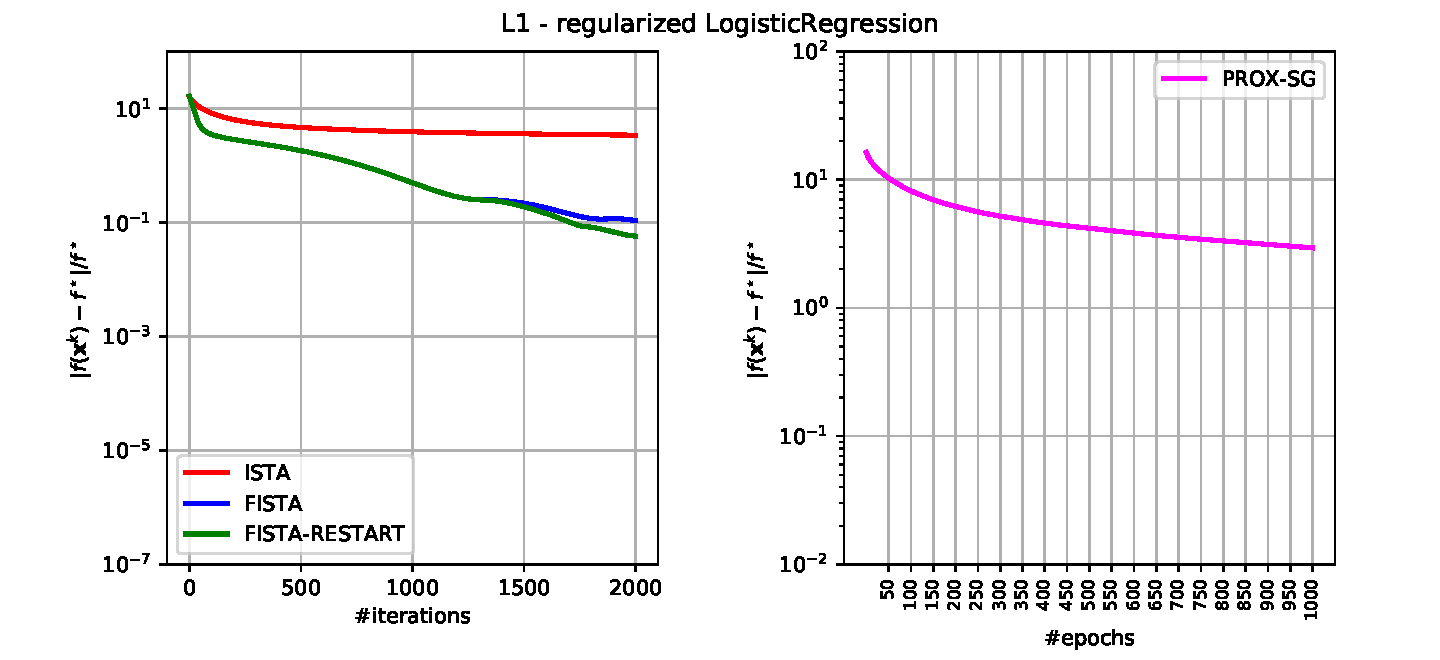
\includegraphics[width=17cm]{hw3/codes/exercise1/results/l1.pdf}
    \caption{Convergence of $\ell$-1 regularized Logistic Regression}
    \label{fig:l1-convergence}
\end{figure}

\begin{figure}
    \centering
    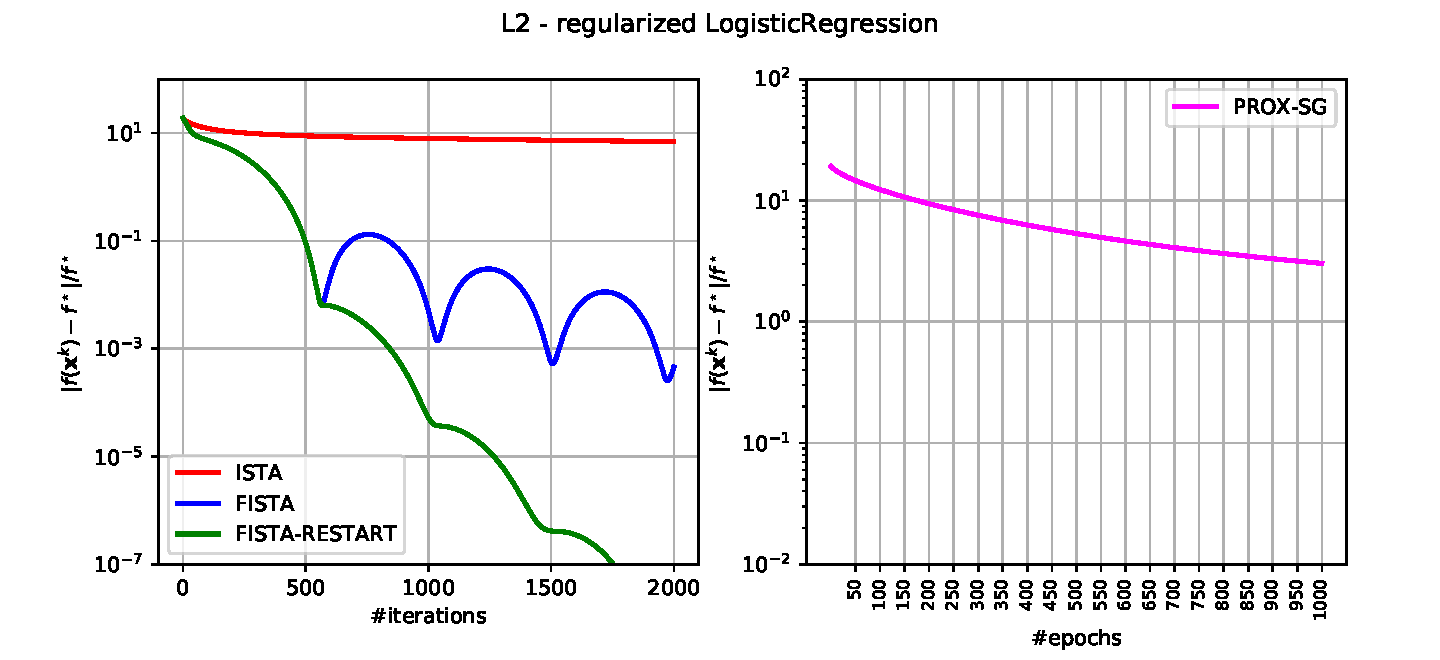
\includegraphics[width=17cm]{hw3/codes/exercise1/results/l2.pdf}
    \caption{Convergence of $\ell$-2 regularized Logistic Regression}
    \label{fig:l2-convergence}
\end{figure}

\begin{figure}
    \centering
    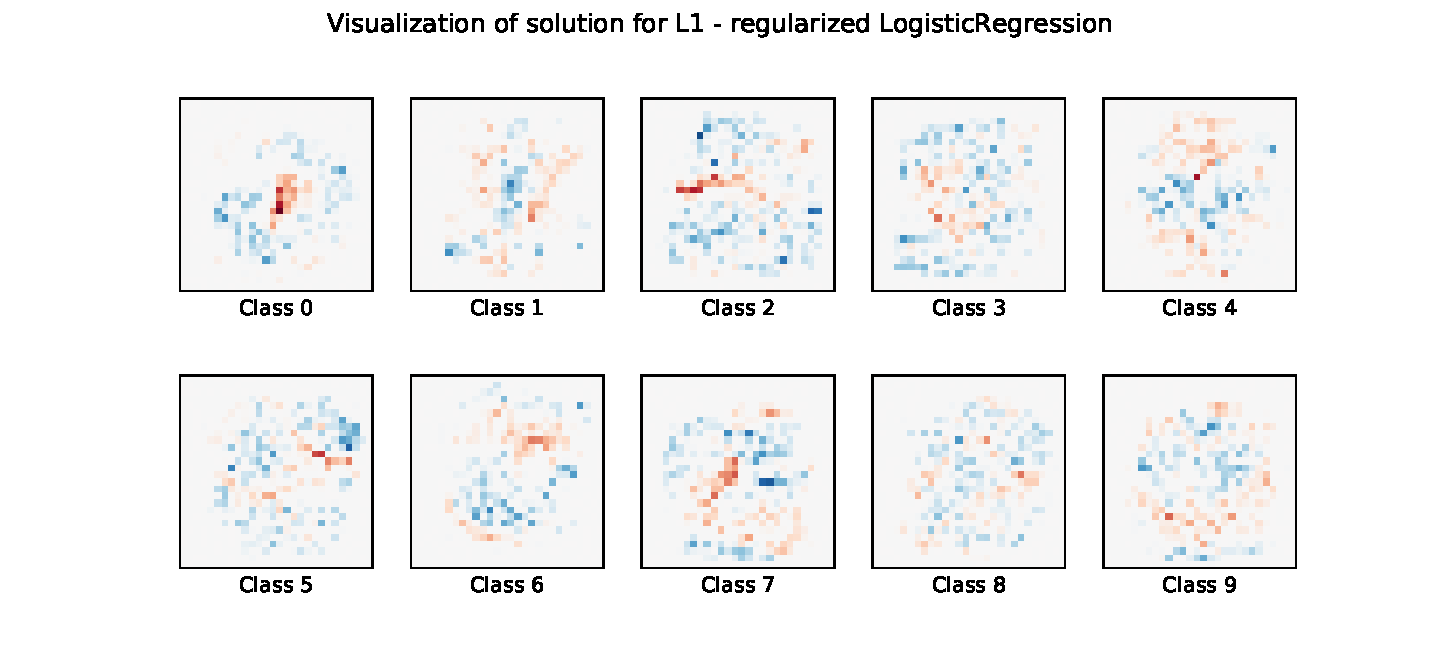
\includegraphics[width=17cm]{hw3/codes/exercise1/results/l1-numbers.pdf}
    \caption{Solution of $\ell$-1 regularized Logistic Regression}
    \label{fig:l1-solution}
\end{figure}

\begin{figure}
    \centering
    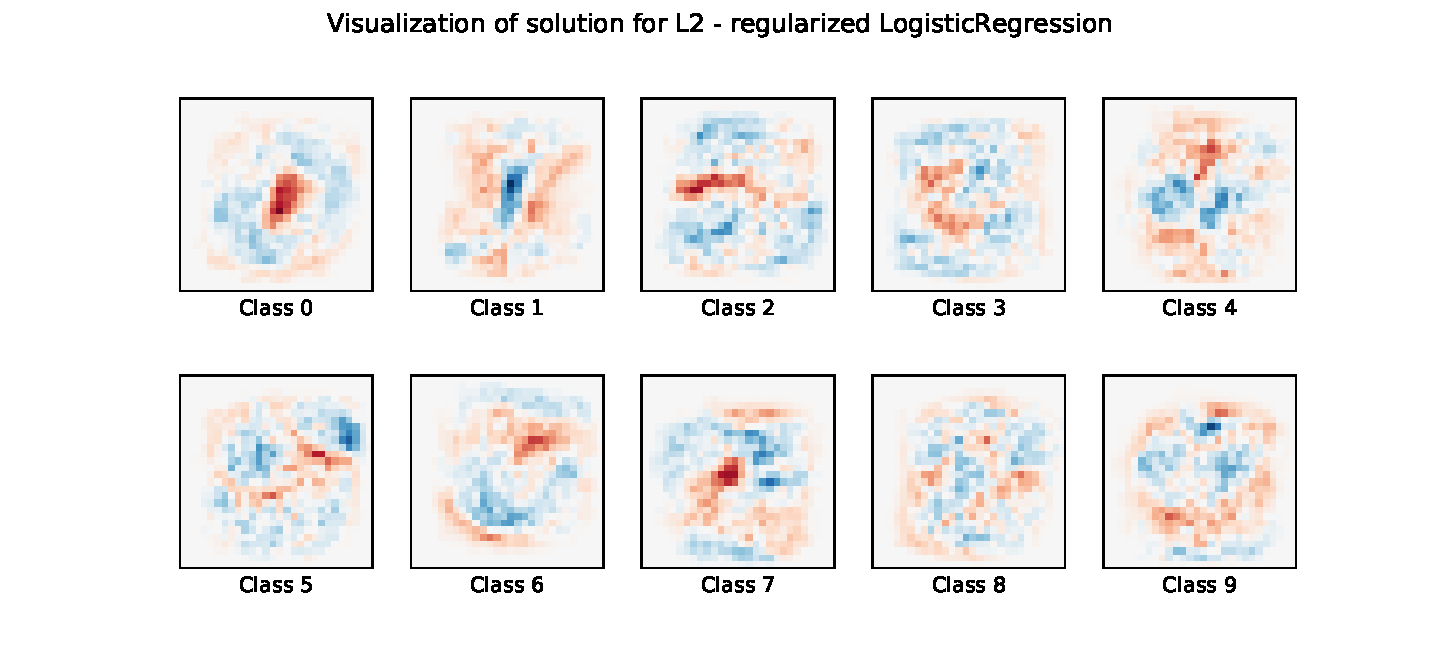
\includegraphics[width=17cm]{hw3/codes/exercise1/results/l2-numbers.pdf}
    \caption{Solution of $\ell$-2 regularized Logistic Regression}
    \label{fig:l2-solution}
\end{figure}

\subsubsection{Logistic Regression and Neural Network comparison}
\begin{itemize}
    \item $\ell$-1 final accuracy = 89.21\%
    \item $\ell$-2 final accuracy = 89.89\%
    \item NN final accuracy = 94.7\%
\end{itemize}

\section{Image reconstruction}
\subsection{Properties of TV and \texorpdfstring{$\ell$}{Lg}-1 in-painting}
\subsubsection{Gradients of TV and \texorpdfstring{$\ell$}{Lg}-1 in-painting}

\subsubsection{Lipschitz constants of TV and \texorpdfstring{$\ell$}{Lg}-1 in-painting}

\subsection{FISTA implementation and \texorpdfstring{$\lambda$}{Lg} sweep}
\begin{figure}
    \centering
    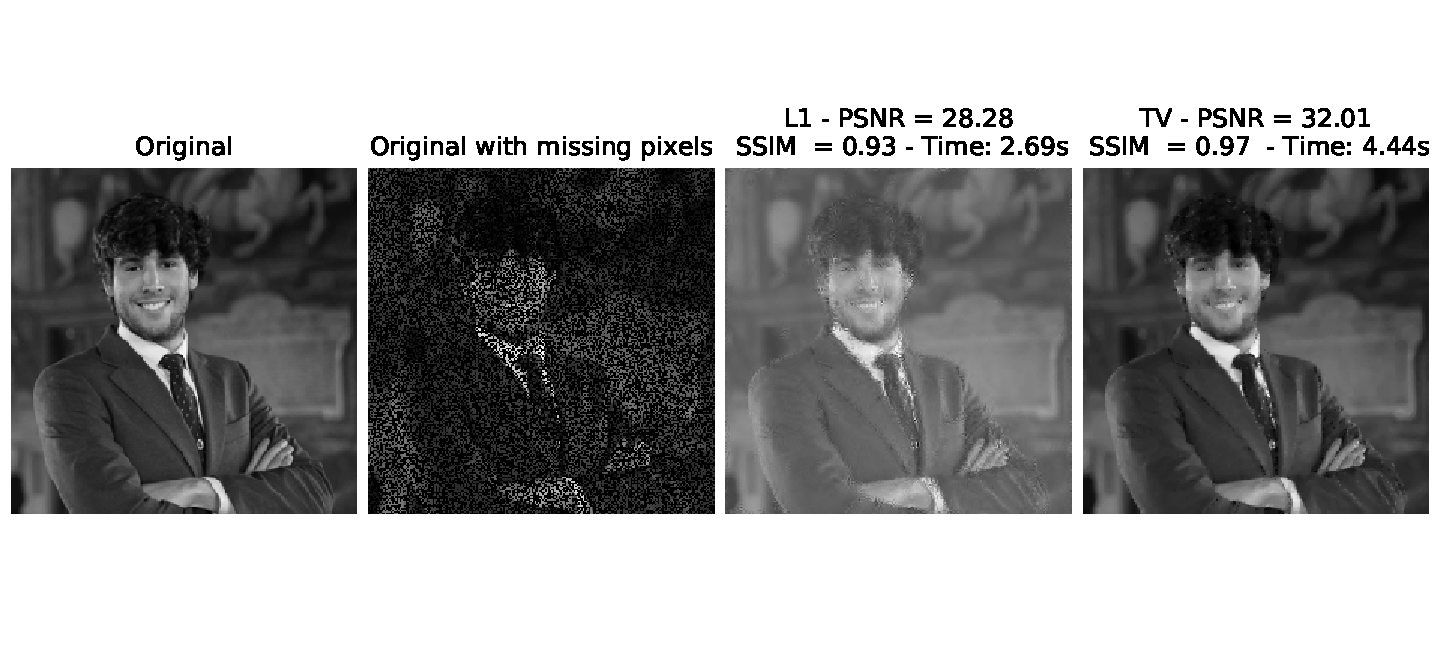
\includegraphics[width=17cm]{hw3/codes/exercise2/results/lambda_search/me_0-001.pdf}
    \caption{Results obtained with $\lambda = 0.001$}
    \label{fig:lambda-search-0.001}
\end{figure}

\subsection{FISTA implementation and \texorpdfstring{$\lambda$}{Lg} sweep}
\begin{figure}
    \centering
    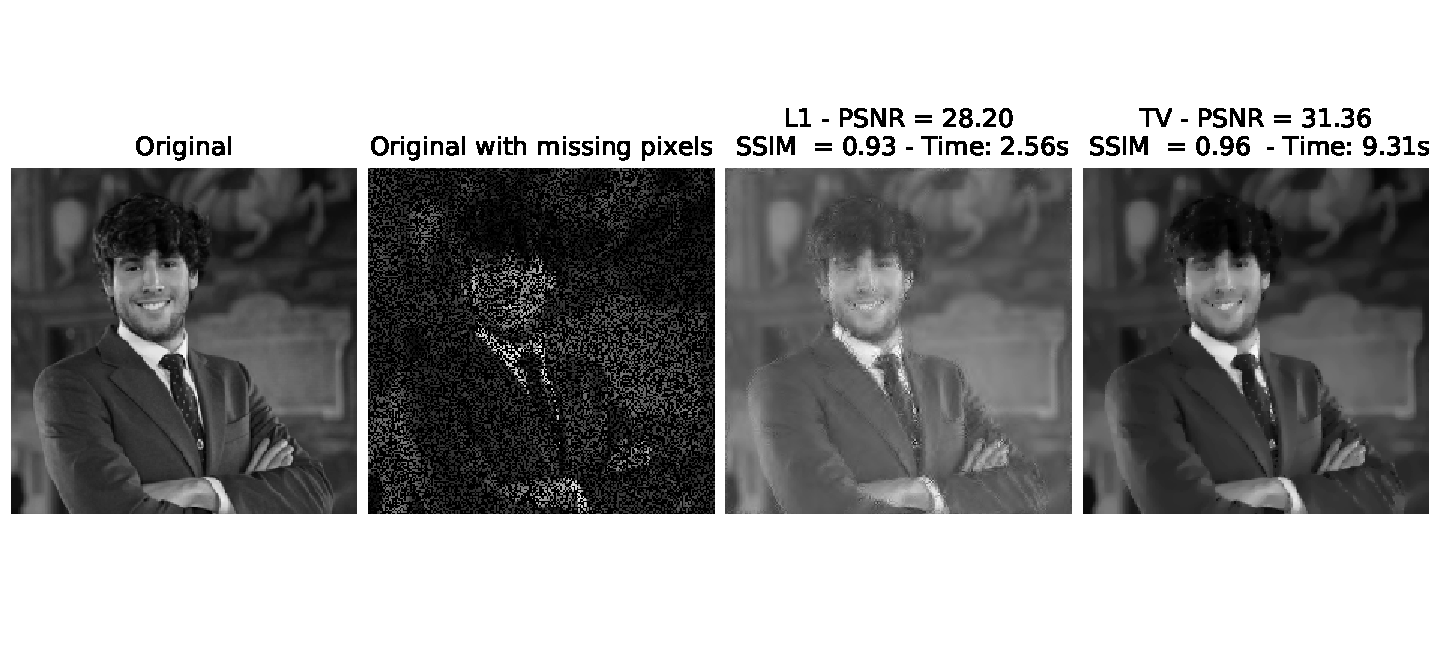
\includegraphics[width=17cm]{hw3/codes/exercise2/results/lambda_search/me_0-01.pdf}
    \caption{Results obtained with $\lambda = 0.01$}
    \label{fig:lambda-search-0.01}
\end{figure}

\begin{figure}
    \centering
    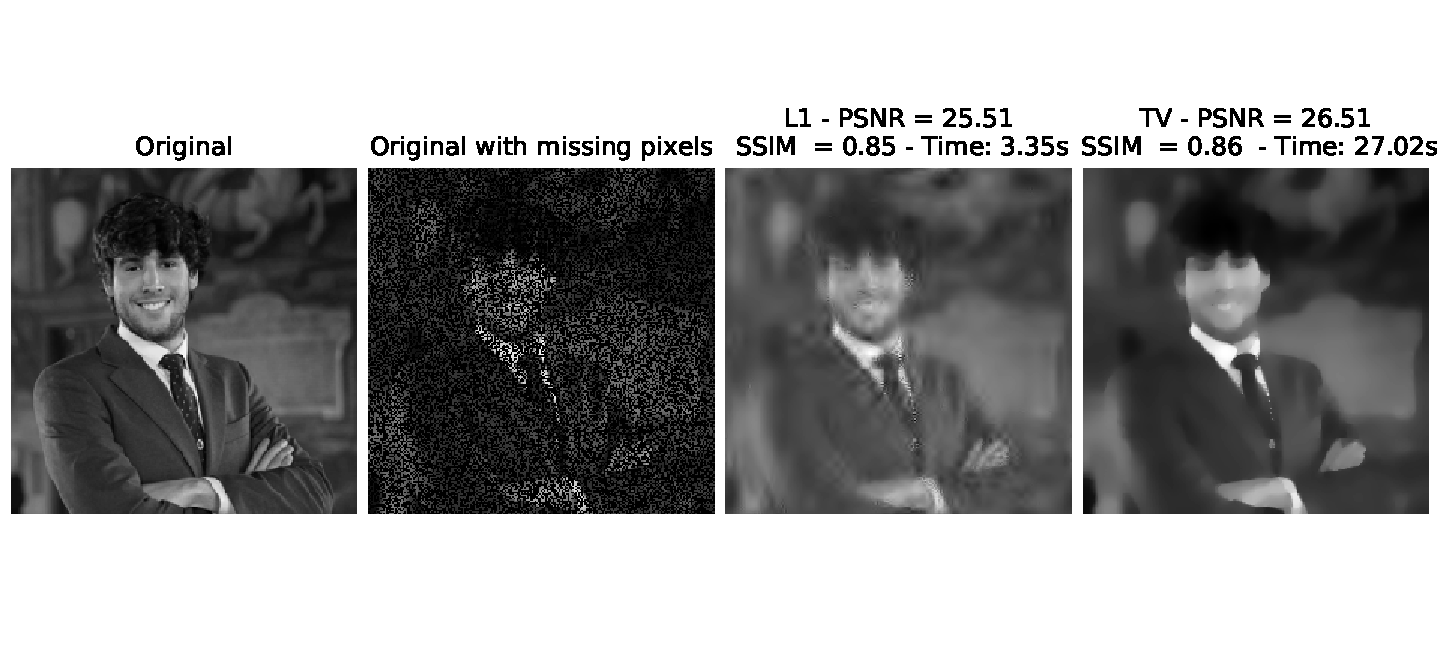
\includegraphics[width=17cm]{hw3/codes/exercise2/results/lambda_search/me_0-1.pdf}
    \caption{Results obtained with $\lambda = 0.1$}
    \label{fig:lambda-search-0.1}
\end{figure}

\begin{figure}
    \centering
    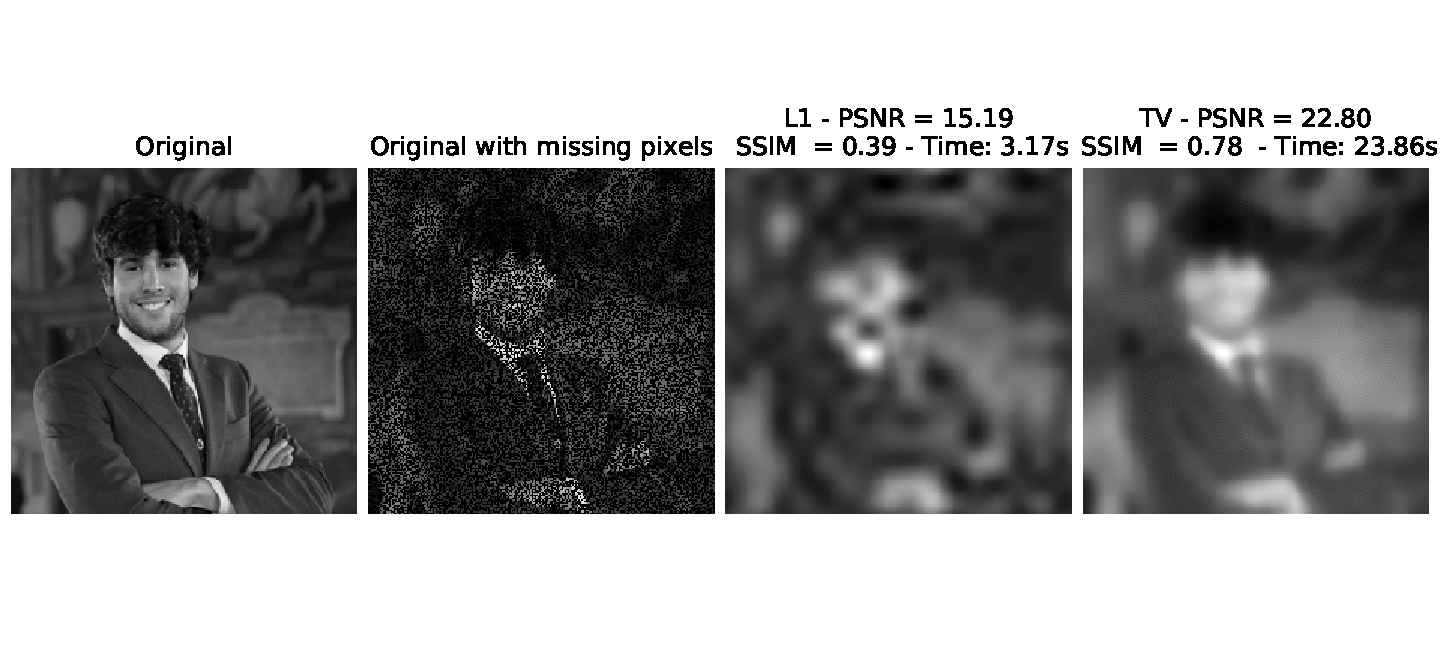
\includegraphics[width=17cm]{hw3/codes/exercise2/results/lambda_search/me_1.pdf}
    \caption{Results obtained with $\lambda = 1$}
    \label{fig:lambda-search-1}
\end{figure}

\begin{figure}
    \centering
    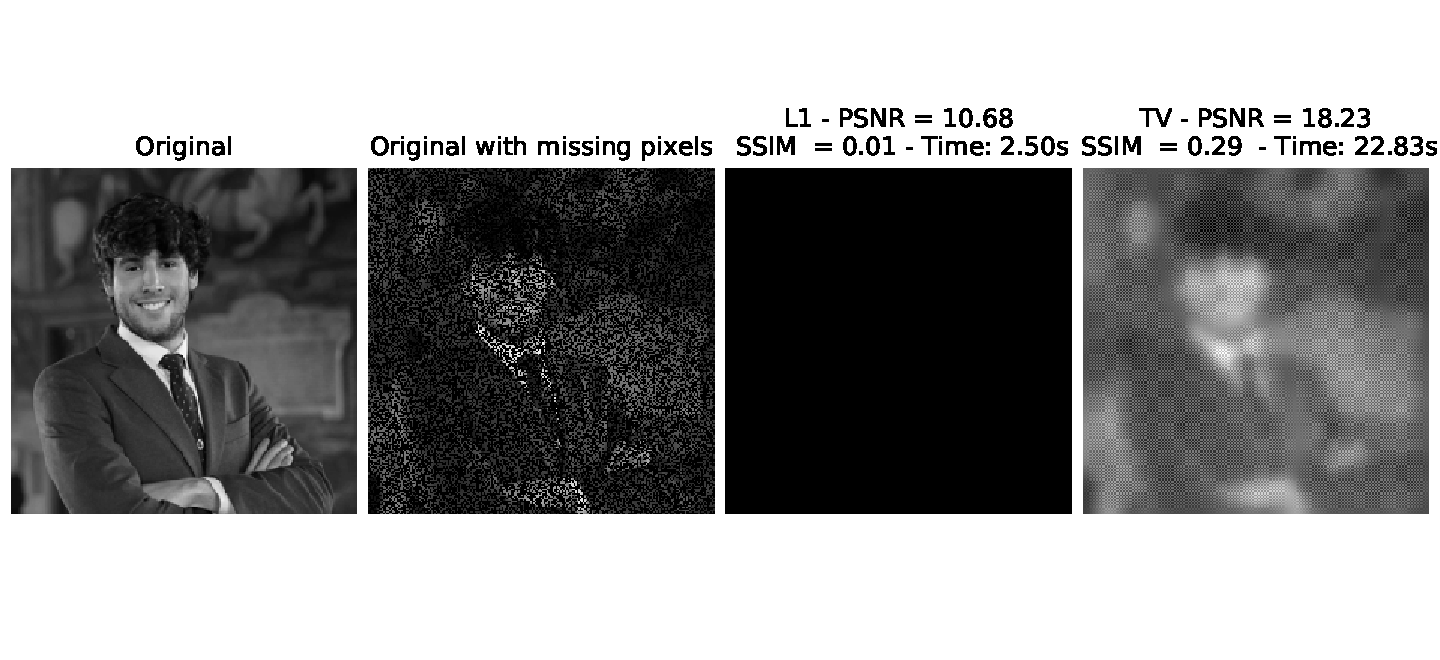
\includegraphics[width=17cm]{hw3/codes/exercise2/results/lambda_search/me_10.pdf}
    \caption{Results obtained with $\lambda = 10$}
    \label{fig:lambda-search-10}
\end{figure}

\begin{figure}
    \centering
    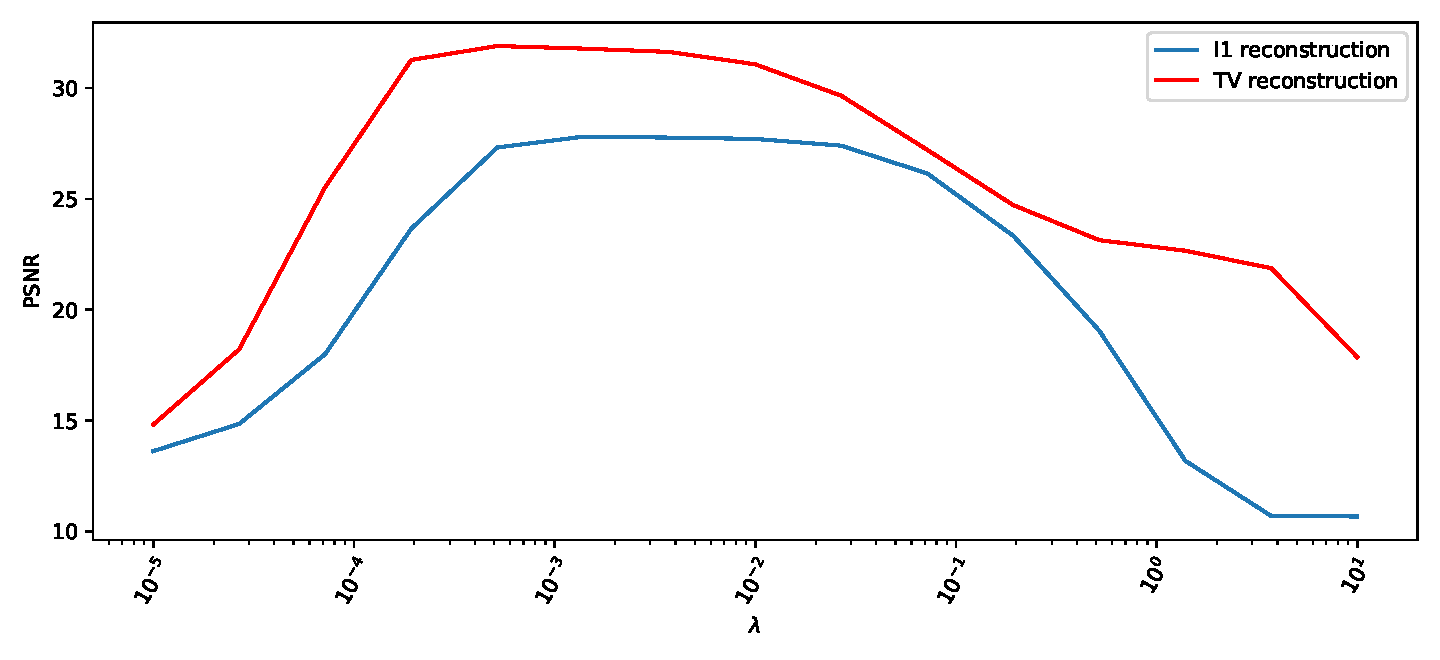
\includegraphics[width=17cm]{hw3/codes/exercise2/results/lambda_search/lambda_search.pdf}
    \caption{PSNR as a function of the regularization parameter $\lambda$}
    \label{fig:lambda-search}
\end{figure}

\subsection{Proximal methods convergence}

\subsection{Wavelet in-painting and NN unrolling comparison}

\end{document}